% Chapter 9

\chapter{Implementation details}
\label{Chapter9}

In this chapter we will focus on the implementation details of the main components and operation, trying to give a clearer idea of the mechanism under the hood of the app. We will start by explaining the general idea and purpose of each included component and their main functions. Then we will move to the sequence flow section, where we will put all pieces together in order to explain their iterations and give a picture of what is happening in the different use cases.

\section{Main components}
We decided to include only, which are for us, the main components of the app, and exclude all the others that are not so relevant in order to understand the operations flow. For the first two, we will start from an abstract idea of the component, identifying the main functionalities that it has to provide.\\
If we think about our application in an high level, it usually will need to acquire the ECG signal from a source, decode and modify it, and finally display it in the screen. This operations are splitted in two components:
\begin{itemize}
	\item A Data Source that will take care about acquisition and decoding
	\item A Display that will take care about all the operation related to drawing ECG signal
\end{itemize}

\subsection{Data Sources}
As introduced before, the Data Source components will take care about receiving the signal from a source, decode and modify it, and pass this information to a Display. Going down of a level, we know that ECG signal in our app will come from:
\begin{itemize}
	\item a saved ECG record file (.dat file), during record opening;
	\item the acquisition device zecg, through a bluetooth connection during real-time acquisition.
\end{itemize}
From this last distinction, we could go down to another level on both possibilities:
\begin{itemize}
	\item in saved ECG record opening, there are potentially different format for encoding the ECG signal in a file;
	\item the acquisition could support many acquisition device, and not only zecg.
\end{itemize}
For these reasons it can be very effective to abstract as much as possible all the characteristics that different acquisition devices or file formats share. In this way we can treat them on the same way in many situations.\\
Actually we were not required to support many different acquisition devices, and the high parametrization of the device in the app settings was quite enough for our goal. For this reason the acquisition will be handled by the class ZEcgReceiver, which does not implement any interfaces or extends any abstract classes.\\
We wanted instead to set that abstraction level for which regards different ECG record format. For this reason we will start from the description of the SampleSource interface, and then we will talk about its implementing abstract class, the DatReader, and finally how to deal with different ECG record formats.

\subsubsection{SampleSource}
SampleSource is an interface that is useful for the saved ECG record opening. It will include methods for getting sample from a source, starting and pausing a ECG playing animation (two types: scrolling or oscilloscope), adding listeners and others. An overview of all methods is given in the figure \ref{fig9.1}.
\begin{figure}[ht!]
	\centering
	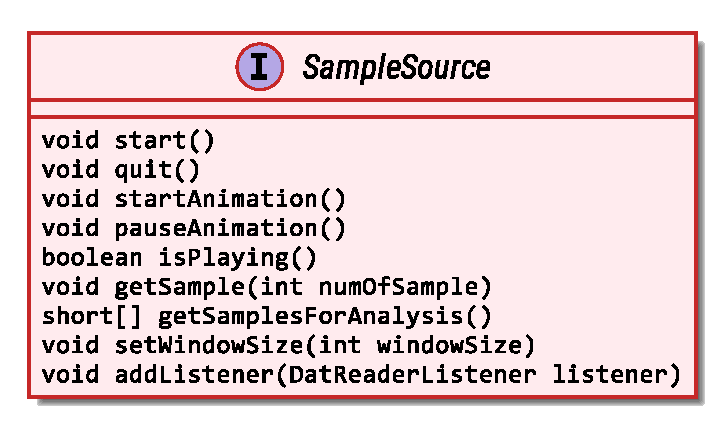
\includegraphics[width=90mm]{figures/ch9/1.eps}
	\caption{Class diagram of the SampleSource interface.}
	\label{fig9.1}
\end{figure}
All its methods are:
\begin{itemize}
	\item start(): it starts the SampleSource and prepare all resources that it needs;
	\item quit(): it stop the SampleSource and destroys all resources used;
	\item startAnimation(): it starts the animation of the ECG signal (scrolling or oscilloscope);
	\item pauseAnimation(): it pauses the animation of the ECG signal;
	\item isPlaying(): it returns true if the animation is active, false otherwise;
	\item getSamples(numOfSamples): it gets from the source numOfSamples samples and stores them;
	\item getSamplesForAnalysis(): it returns D2 lead, used for the ECG analysis;
	\item setWindowSize(windowSize): it sets the size of the display window size, specified in number of samples, that depend on the device screen size and orientation;
	\item addListener(listener): it registers a listener that will be notified if the SampleSource changes animation state.
\end{itemize}
The SampleSource interface that we introduced will be the basis for the following class description, the DatReader, the core of our record ECG opening.

\subsubsection{DatReader}
The DatReader is an abstract class that handles all the most sensitive operations for which regarding ECG record opening. It implements the SampleSource interface, described before, and permits to support many kind of ECG record format, with the only need of overriding one of their methods. There are many things under the hood of this class, so they will be described one by one.\\
The first characteristic of this class is that, all its operation are executed asynchronously from the UI thread: this is done by extending the class HandlerThread, described in the previous chapter. By doing this, we can exploit all the functionalities provided by this class, as the Looper and Message passing mechanism. So the DatReader once started, it will stay watching at its MessageQueue, though its Looper, waiting for a new message. The messages in this class will be basically the number of samples that it will need to read. To read the ECG samples, the DatReader will hold a stream to the record .dat file (file containing all samples). Reading constantly from a file, therefore avoiding the allocation in memory of the record, permits us to maintain the app memory low.\\
But who is sending these messages to the DatReader? Well, there are basically two scenarios:
\begin{itemize}
	\item The user that is using the app scroll the ECG paper with its finger, causing the app to load the right number of samples depending on the movement size and direction;
	\item The user activated the ECG scrolling animation, and so some samples need to be loaded after a certain period, depending on the ECG record rate.
\end{itemize}
Focusing on the first scenario, the entity that will handle ECG visualization and user inputs will be the SampleDisplay, which will be described in details in the next section. And so it will respond to the user scroll, calculating the right number of samples and request them to the DatReader, which is viewed as a SampleSource. The request will be represented by a Message, containing all useful information, like of course the number of samples to load, but also others.\\
There is a problematic where we want to provide scrolling of the ECG paper in both direction, while we are reading constantly from a file: we need to be able to move the file pointer in both direction, not a trivial functionality. The class that we rely on is the RandomAccessFile class: using this class we can always retrieve the actual position of the file pointer and then move it with the method seek(). But this is not the only problematic. We need to take into account that the application will always show on screen a window of the ECG record, with a dynamic size, dependent on the space available on screen. Therefore, the file pointer will refer to a specific point of this window. This point can be the tail or the head of the window, namely the point where the samples were added last time.\\
Consider the following example, represented in the figure \ref{fig9.2}: an user opens a ECG record, the DatReader will be created and started, and will load all the samples need in order to fill the device screen. At this moment, it will have read all the samples sequentially, from the first one to the the last required one, from the file. Thus, the file pointer is referring to the tail of the ECG record window. After that, the user starts scrolling to the right, in order to see the following two seconds of the record. So the DatReader continues to read sequentially the following samples in the file. But now suppose that the user decides to change its scrolling direction and go back. We cannot only read the file backwards from the last pointer position, because those samples will be already loaded and visualized in the sample window. What we need to do is to skip the entire window, and start reading from that point. So after the left scroll, the pointer will be moved to the head of the window.\\
\begin{figure}[ht!]
	\centering
	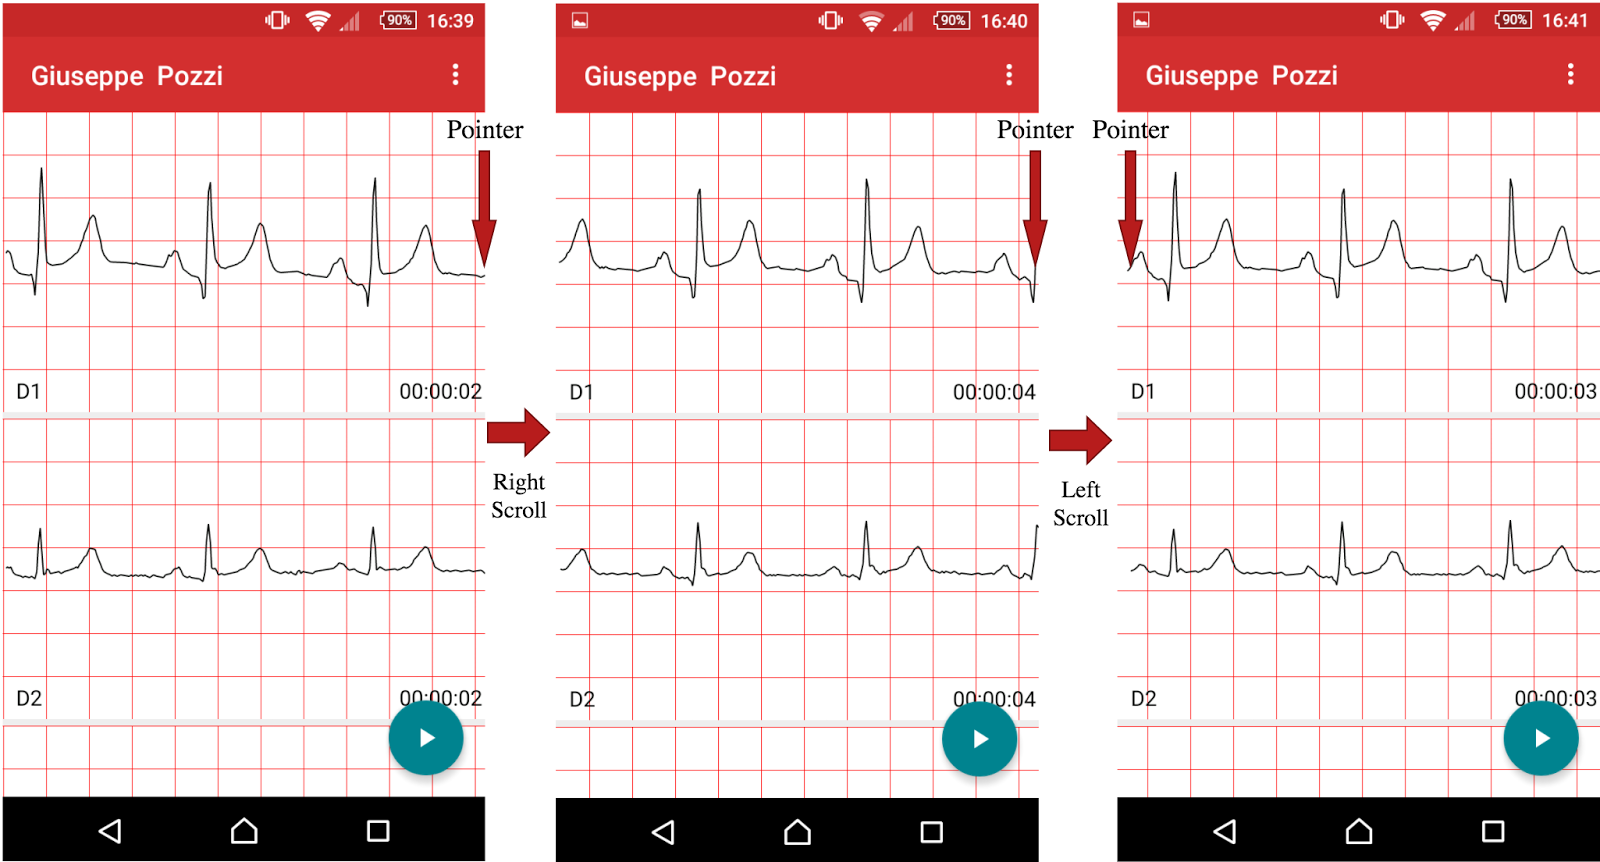
\includegraphics[width=140mm]{figures/ch9/2.png}
	\caption{The movement of the file pointer in the DatReader, after the user change direction of scrolling the ECG paper.}
	\label{fig9.2}
\end{figure}
To make this mechanism possible, it is clear that we have to store the previous reading direction, stored in the variable prevDirection. If the new direction will be different, the DatReader will move the file pointer, skipping the window. So we need also to store the size of the window: this is done with the variable windowSize.\\
After each file reading operation, the DatReader will send to the SampleDisplay all new samples, specifying if add them to the tail of the window or to the head. The iteration between  SampleSource and SampleDisplay in the user scrolling scenario is summarized in the figure \ref{fig9.3}.
\begin{figure}[ht!]
	\centering
	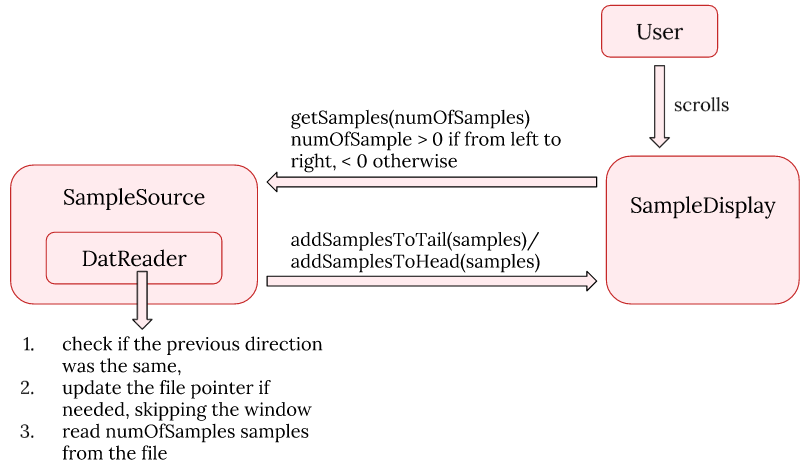
\includegraphics[width=120mm]{figures/ch9/3.png}
	\caption{The iteration between  SampleSource and SampleDisplay after the user scroll the ECG paper.}
	\label{fig9.3}
\end{figure}
Before being sent to the SampleDisplay, the read samples are reconverted to mV, by dividing all values by the gain of the signal. In this way, we can work with universal values during plotting, as different ECG record can have different gain.\\
Now we will move to the second scenario. Here, the user has activated the ECG scrolling animation, by clicking on the play button, which will be binded to the SampleSource, causing the call of startAnimation(). In this case, there will be another entity that will request samples from the SampleSource. The crucial aspect is that, it will continuously requests new samples, but doing so respecting the rate of the original ECG record. This is not a trivial problem, as some requests could be delayed because of another operation that is not finished. So these requests need to be concurrent, reliant on a mechanism to guarantee the right rate, with a good precision. The solution was the adoption of a SheduledThreadPoolExecutor, a pool of thread that we have described in the chapter about concurrency. Thanks to its method:
\begin{lstlisting}
	scheduleAtFixedRate(Runnable command, long initialDelay,
	long period, TimeUnit unit)
\end{lstlisting}
we can program all the requests in the pool by:
\begin{lstlisting}
	scheduledThreadPoolExecutor.scheduleAtFixedRate(new Runnable() {
		@Override
		public void run() {
			getSample(1);
		}
	}, 0, 1000000 / rate, TimeUnit.MICROSECONDS);
\end{lstlisting}
having a precision of microseconds. Being this type of operation not so expensive, we initialized our pool with only one thread.\\
We have omitted that the method getSamples(numOfSamples) doesn’t have an implementation for getting the samples from the source, but it just acts like a request to the SampleSource: by executing it, the implementation in the DatReader will create a message and enqueue it to its MessageQueue. The DatReader will continuously read messages from its MessageQueue and sooner or later, it will find that message, read the sample from the source, and update the SampleDisplay with the new sample. An summarization of the mechanism is showed in the figure \ref{fig9.4}. Furthermore, in the figure \ref{fig9.5}, you can find an overview of the DatReader class, including all variables introduced in this section.
\begin{figure}[ht!]
	\centering
	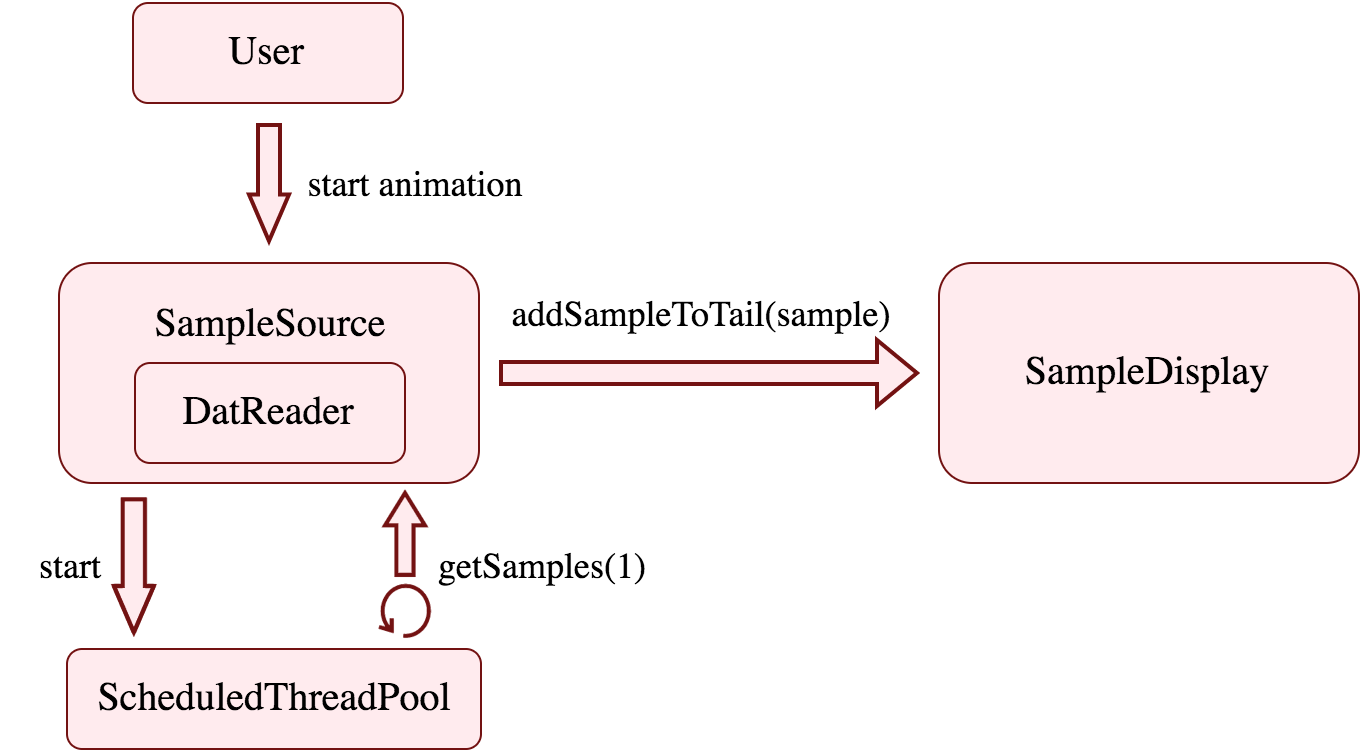
\includegraphics[width=120mm]{figures/ch9/4.png}
	\caption{The animation mechanism of DatReader using SheduledThreadPoolExecutor.}
	\label{fig9.4}
\end{figure}
\begin{figure}[ht!]
	\centering
	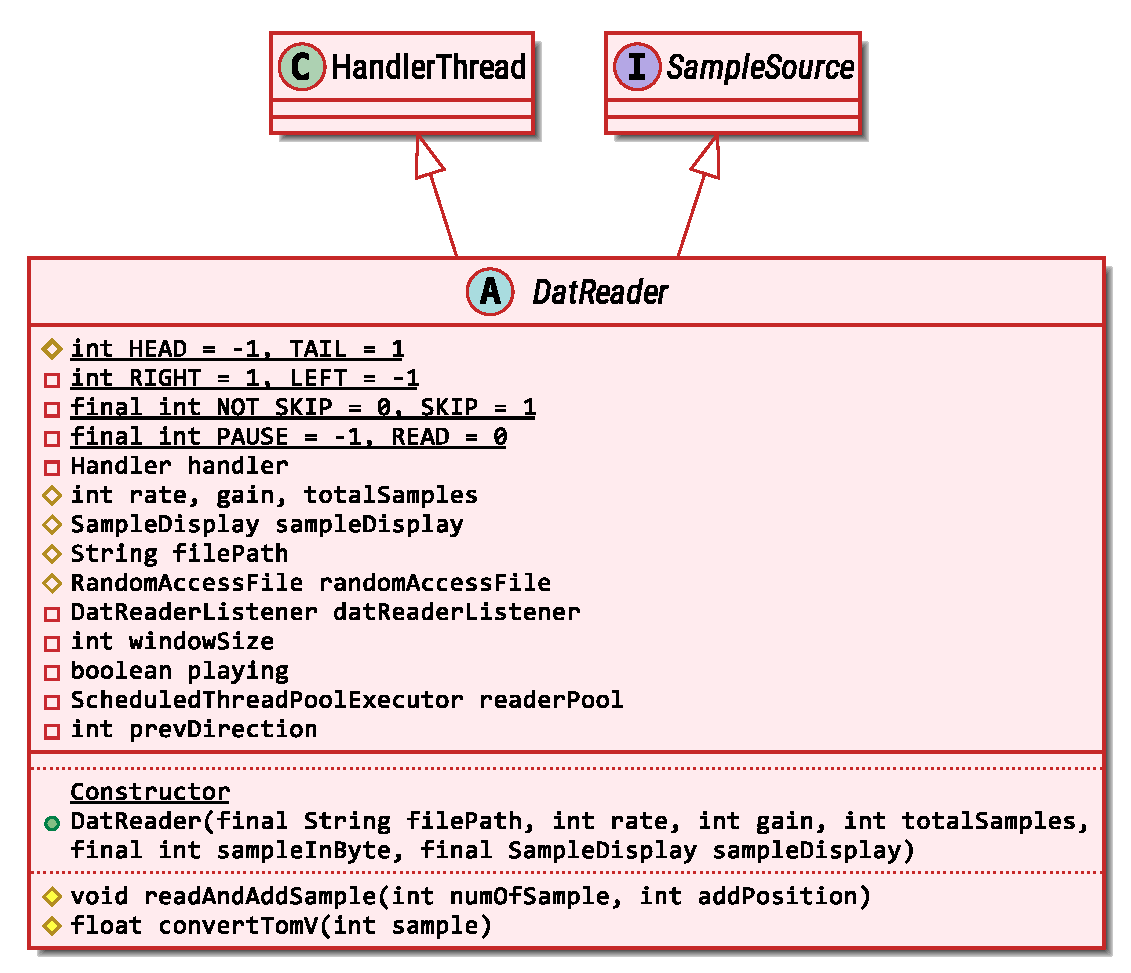
\includegraphics[width=130mm]{figures/ch9/5.eps}
	\caption{Class diagram of the DatReader class.}
	\label{fig9.5}
\end{figure}

\subsubsection{ ZEcgReceiver}
Now we describe the component that will be used during the ECG real-time acquisition. It will communicate with the BluetoothSerial class and interact, similarly to the DatReader, with the SampleDisplay. As the DatReader, it extends the HandlerThread, therefore it will have a personal Looper and MessageQueue. It will also have an acquisitionBuffer that will use to store partial data received from BluetoothSerial. So, what it will do is waiting for new messages on its MessageQueue, and react on a new message. A message coming from BluetoothSerial will contain a buffer of data received from the acquisition device through a bluetooth connection. At a new message receiving , ZEcgReceiver will read the buffer in the message and append it to its acquisitionBuffer. After that,  it will scan its acquisitionBuffer and read all possible samples inside, and free it from all decoded samples. All new decoded samples are then sent to the SampleDisplay for the visualization.\\
ZEcgReceiver will also handle many other operation as:
\begin{itemize}
	\item It will store a heartRateBuffer of the last sample received, with a size of 10 seconds, used to compute the real-time heart rate, to be notified to the SampleDisplay;
	\item It will include the calculation of the Moving Average Filter, if enabled, in order to remove the baseline wander artifact;
	\item The data received from the acquisition device will also include information about its battery level. For this reason, it will parse it and send it to the SampleDisplay;
	\item It will write additional information in the file .hea of the ECG record. 
\end{itemize}

\subsection{Display}
Before we described all the entities behind the generation of the data that will be sent then to the visualization part of the application. Now we will talk about all the components that make ECG visualization possible. Equivalently to the previous section, we will start describing the general interface the will represent the visualization component, the SampleDisplay, moving later to the component that will implement it.

\subsubsection{SampleDisplay}
The have already mentioned many time the SampleDisplay component when talking about data sources. This interface represent the general entity that expose some entry point to add new samples and handle ECG signal visualization. The figure \ref{fig9.6} shows an overview of all methods.
\begin{figure}[ht!]
	\centering
	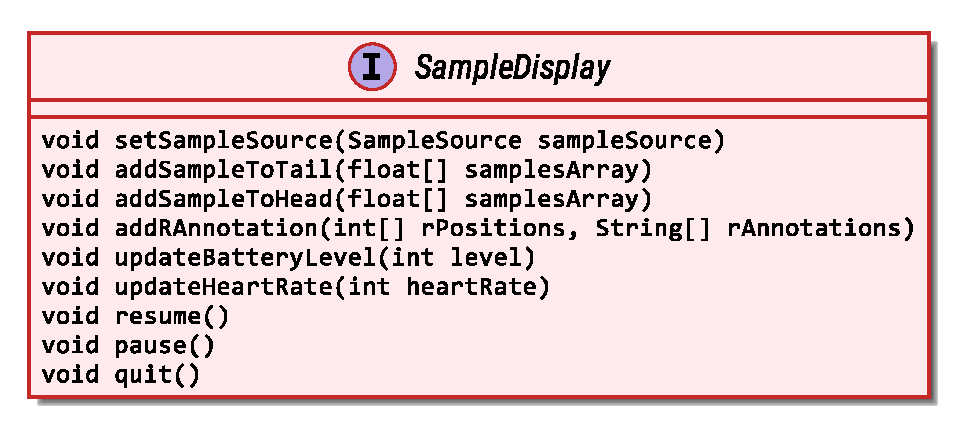
\includegraphics[width=120mm]{figures/ch9/6.eps}
	\caption{Class diagram of the SampleDisplay interface.}
	\label{fig9.6}
\end{figure}
Methods description:
\begin{itemize}
	\item setSampleSource(SampleSource sampleSource): it binds the SampleSource passed as parameter;
	\item addSampleToTail(float[] samplesArray): it adds all samples in the passed array to the tail of the visualized samples window;
	\item addSampleToHead(float[] samplesArray): it adds all samples in the passed array to the head of the visualized samples window;
	\item addRAnnotation(int[] rPositions, String[] rAnnotations): it stores all the R position ( of the QRS complex ), with their relative annotations coming from the ECG signal analysis;
	\item updateBatteryLevel(int level): it updates the visualized battery level;
	\item updateHeartRate(int heartRate): it updates the visualized heart rate in BPM;
	\item resume(): it resumes the ECG signal visualization;
	\item pause(): it pauses the ECG signal visualization;
	\item quit(): it will close and free all the components used for visualization.
\end{itemize}

\subsubsection{SignalScrollView}
For our visualization of the ECG signal we wanted to provide a scrollable view of different ECG paper strip, where in each one was displayed a different ECG lead. Hence, we selected as entity implementing the SampleDisplay interface, a customized version of the ScrollView class, a scrollable view provided in Android. This class will be the entry point for all data sources, and a container for some other components, described in details further on. These contained elements will be the all SignalSurfaceViews, where each one represent the view of an ECG lead. The SignalScrollView represents also the core for one of the feature described in the previous chapters: the dynamic display scaling. It will do all calculation inside its method calculateMetrics(). The goal of the method is calculate the size of the basic block of the standard ECG paper, which is 0.5 cm, in pixel. The problem is that the pixel size varies a lot, being dependent on the device screen pixel density. So for doing this, we need to retrieve the pixel density of the device screen, and then calculate properly the right size of the blockInPixel( figure \ref{fig9.7} ). 
\begin{figure}[ht!]
	\centering
	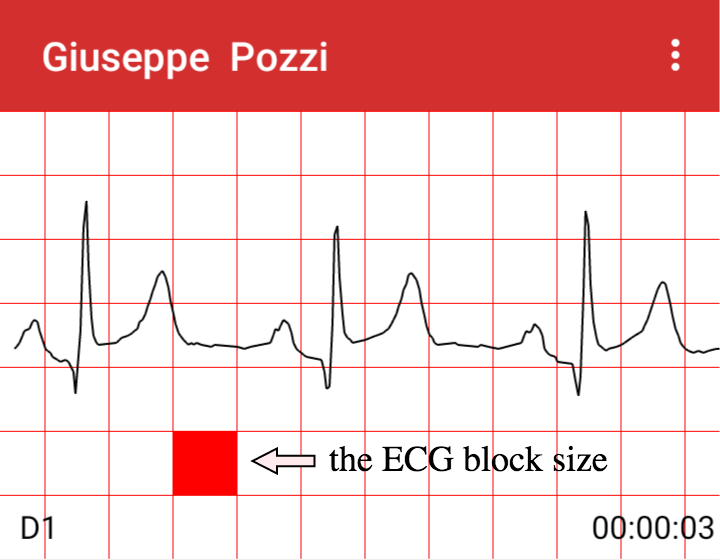
\includegraphics[width=90mm]{figures/ch9/7.png}
	\caption{The size of the ECG paper block after the computation of the method calculateMetrics().}
	\label{fig9.7}
\end{figure}
The measure used to represent the pixel density is the \textit{dpi (dots per inch)}, defined as \textit{“the number of individual dots that can be placed in a line within the span of 1 inch (2.54 cm)”}.\cite{ref24} The formula for the computation of the blockInPixel will be:
\begin{equation}
	blockInPixel=\frac{dpi*blockInCm}{inchInCm}
\end{equation}
where:
\begin{itemize}
	\item \textit{dpi}: screen pixel density, dependant on the device specification;
	\item \textit{blockInCm}: the size of the ECG paper block in centimeters, equals to 0.5 cm;
	\item \textit{inchInCm}: the size of one inch in centimeters, equals to 2.54 cm.
\end{itemize}
With this calculation we can ensure a perfect scaling in many device, with a very small error percentage for high pixel density screens ( $\sim$240dpi or higher ).\\
The method calculateMetrics() take place in the initialization process of the class, together with the method fillScrollView(int heightInBlock). This method receives the parameter heightInBlock, which comes from the app settings and specifies the height of the ECG paper strip in ECG standard blocks, and create and add inside the SignalScrollView all the SignalSurfaceViews needed, depending on the number of ECG signal leads (one per lead). Moreover, during its initialization, the class will create another important component, the DrawingHelper, that we will describe next. This last will handle all the call of the SampleDisplay methods:
\begin{itemize}
	\item addSampleToTail(float[] samplesArray);
	\item addSampleToHead(float[] samplesArray).
\end{itemize}
For this reason, SignalScrollView will route each adding request to the DrawingHelper, that will take care of storing the visualize samples window and adding all new samples to it.\\
Furthermore, SignalScrollView will perform a very important optimization for the visualization of the ECG paper strip: with its method pauseNotVisibleView() will be able to select only the strips that are present in the screen, and pause the drawing routine ( described in the next sections ) for all not visible strips, saving lot of computational power. This method will be triggered every time the user will scroll the view.\\
Lastly, we need to specify that SignalScrollView will also handle drag events coming from the user when he wants to scroll the ECg paper. But the class will be used as reference class both during real-time acquisition and ECG record opening. The difference in these scenario is that, during real-time acquisition, the dragging need to be disabled, while in the other, enabled. So to achieve this distinction, inside the constructor will be passed the parameter dragEnabled, which will be used to activate or not the overridden method onTouchEvent(MotionEvent ev), that will take care about decode the performed scroll and notify the SampleSource.\\
	As usual, an overview of the class could be seen in the figure \ref{fig9.8}.
\begin{figure}[ht!]
	\centering
	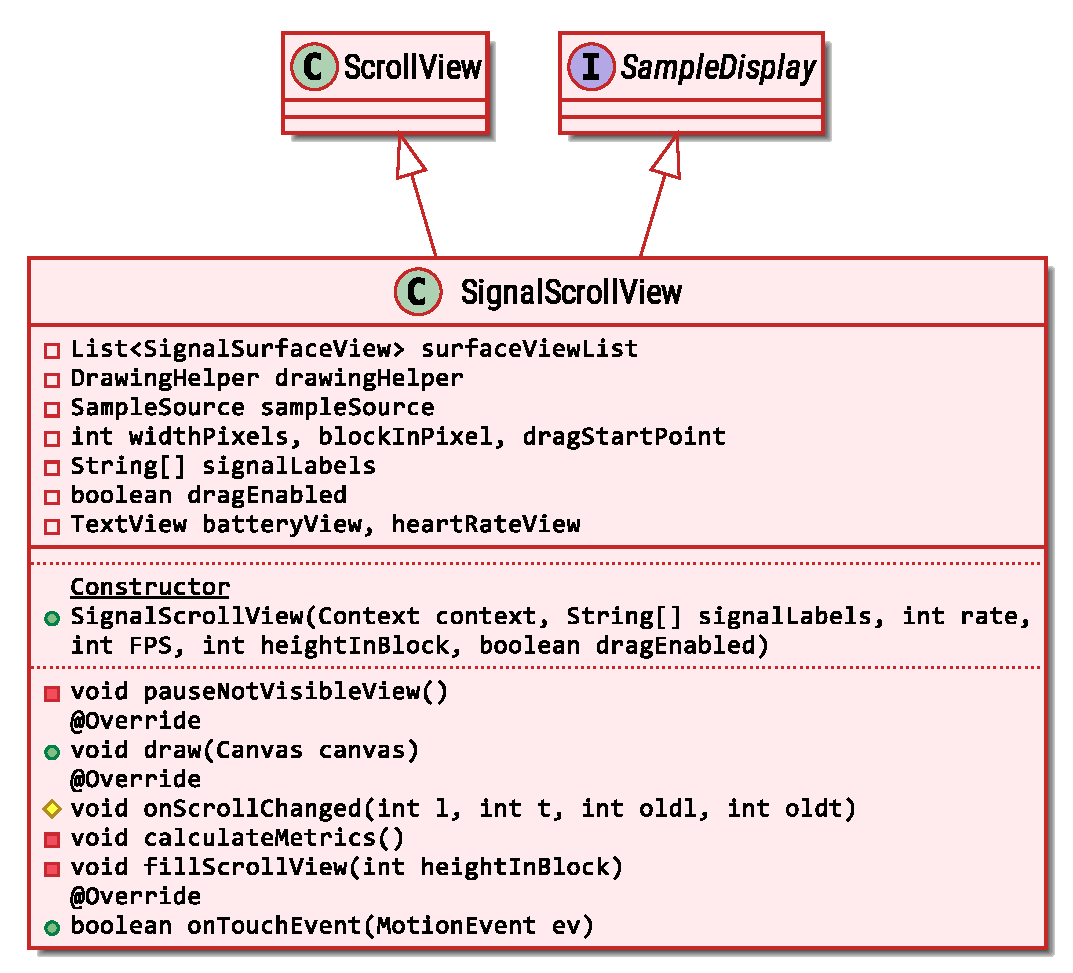
\includegraphics[width=130mm]{figures/ch9/8.eps}
	\caption{Class diagram of the SignalScrollView class.}
	\label{fig9.8}
\end{figure}

\subsubsection{SignalSurfaceView}
In  order to achieve the best performance, we used the best mechanism available in Android for fast and custom drawing. For this purpose we extended the class SurfaceView. As explained in the Android developer site \textit{“The SurfaceView is a special subclass of View that offers a dedicated drawing surface within the View hierarchy. The aim is to offer this drawing surface to an application's secondary thread, so that the application isn't required to wait until the system's View hierarchy is ready to draw. Instead, a secondary thread that has reference to a SurfaceView can draw to its own Canvas at its own pace.”}\cite{ref25}. We will focus on the thread responsible of drawing on the SignalSurfaceView when will describe the Drawer class. For now, we describe only the main operation of the SignalSurfaceView. This class will be liable of reacting after the creation of the view and on view change event. This last will occur typically after a rotation of the device screen, performed by the user. This will cause for example to change the orientation from portrait to landscape, and so the new SignalSurfaceView will be required to fill all the new available space.

\subsubsection{DrawingHelper}
As the name suggests, this is the helper class for all drawing operation. Many of its methods and variables will be used by the Drawer for handle drawing. It is an abstract class, because we provide to different plotting type: a scrollable drawing and a oscilloscope drawing ( figure \ref{fig9.9}). For each type, there is a proper extending  class:
\begin{itemize}
	\item DrawingHelperScroll, for scrollable drawing type;
	\item DrawingHelperOsc, for oscilloscope drawing type.
\end{itemize}
\begin{figure}[ht!]
	\centering
	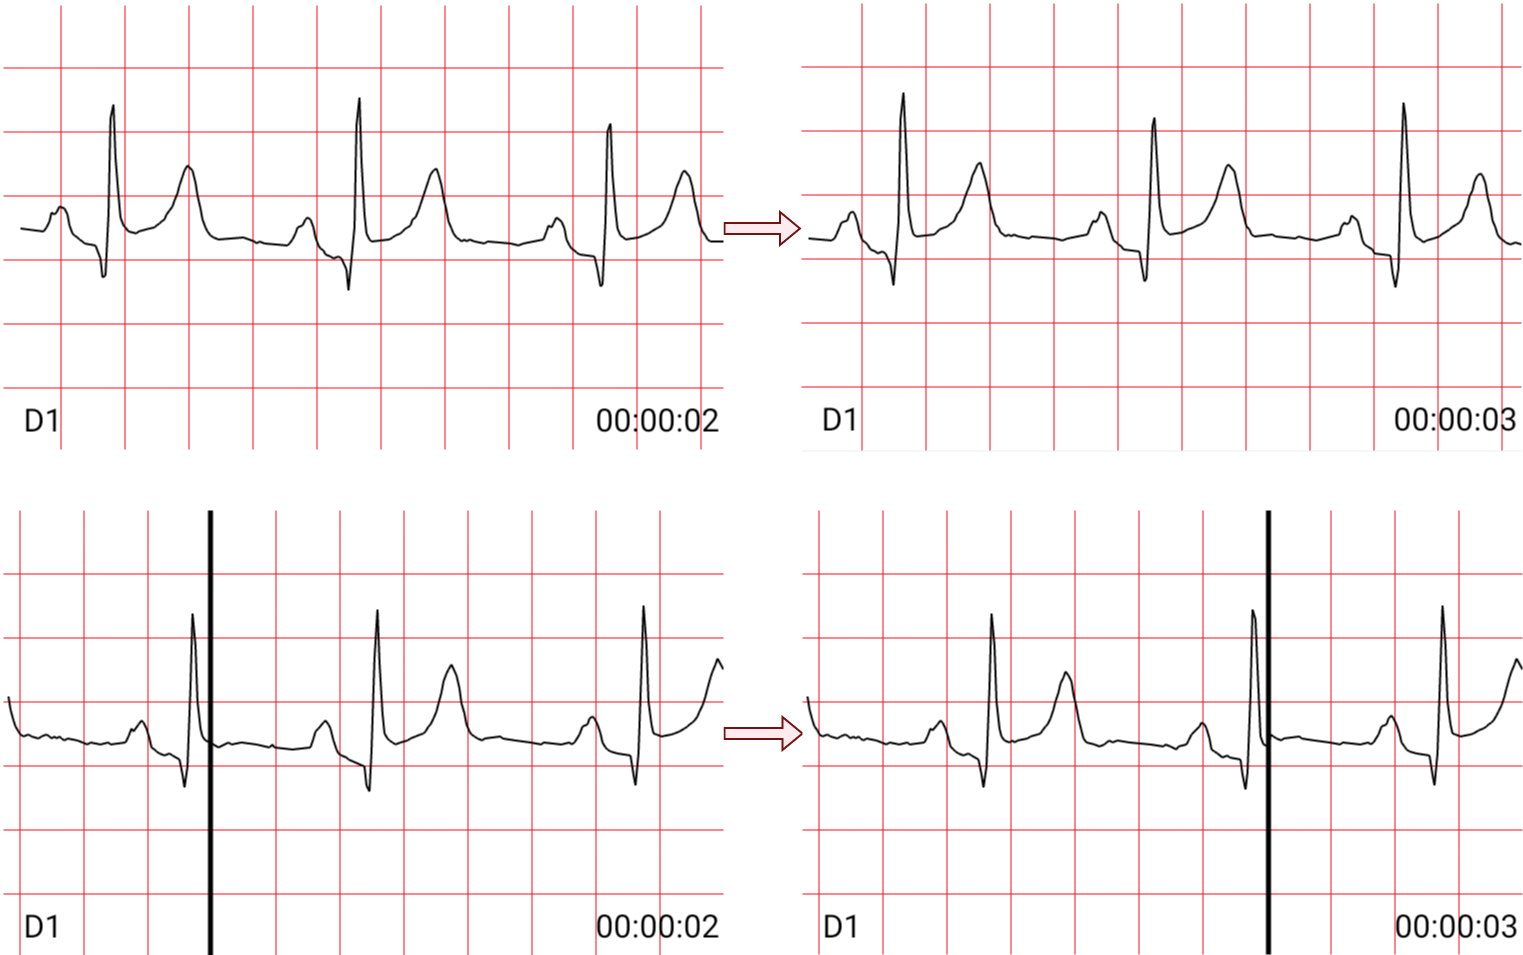
\includegraphics[width=100mm]{figures/ch9/9.png}
	\caption{The different ECG visualization types. The one on top is the scrolling drawing, the one in the bottom is the oscilloscope drawing. The time elapsed after the movement of the ECG paper is one second.}
	\label{fig9.9}
\end{figure}
Each of these class will store the list of all sampleWindows, containing a sampleWindow for each ECG lead. The sampleWindow will store the samples window that is currently visualized on the screen. The collection type for the sampleWindow is different in the two classes, because each one use the most suitable implementation for its update type. For example, the DrawingHelperScroll, will treat the window as a queue: it will always add new sample to the head or to the tail. Thus, it uses a ArrayDeque, an very efficient and fast class when applied to this type of scenario.\\
During its initialization, with the method prepare(args ...) the DrawingHelper creates some Drawer. This last is the class used for drawing on the SignalSurfaceView, and will be described in the next section. The number of Drawer created depends on the computational power availability of the device used: in the method the DrawingHelper will retrieve the number of cores available in the device CPU, and will create accordingly the same number of  Drawer ( which, you will see, will extend the HandlerThread class ). For this reason, with a single core CPU, only a Drawer will be created, and it will be the sole handler for all the SignalSurfaceView ( and so all ECG strips ). Instead, if we had four CPU core, and for example all the twelve ECG leads, there will be created four Drawer, where each will handle the drawing of three SignalSurfaceView. This characteristic provide a nice performance scalability, dependent on the CPU of the used device.\\
The DrawingHelper also will handle the lifecycle of all Drawers using:
\begin{itemize}
	\item startDrawing(int signalIndex), for starting the drawing operation of the Drawer which is the handler for the passed signalIndex;
	\item pauseDrawing(int signalIndex), for pausing the drawing operation of the Drawer which is the handler for the passed signalIndex;
	\item quit(), for stopping all Drawers currently active and destroying them.
\end{itemize}
Furthermore, the DrawingHelper will provide the helper methods, used by the Drawer, to compute the different drawing layers:
\begin{itemize}
	\item drawGrid(Canvas c, Paint p): it draws the ECG grid in the passend Canvas using the passed Paint. It uses the variable blockInPixel for the right sizing;
	\item drawSignalLabelsAndTime(int signalIndex, Canvas c, Paint p): it draws the labels of the time and the ECG leads in the passend Canvas using the passed Paint;
	\item drawSamples(int signalIndex, Canvas c, Paint p): it draws all the samples inside the sampleWindow as lines in the passend Canvas using the passed Paint. It avoid the drawing of consecutive equals value when plotting the lines, in order to save useless operations;
	\item drawRAnnotations(Canvas c, Paint p): it highlights all the R peaks by drawing vertical lines on them and with the respective R annotation, in the passend Canvas using the passed Paint. This of course will be active only after the analysis.
\end{itemize}
In the figure \ref{fig9.10} you can find the class diagram of the DrawingHelper class.
\begin{figure}[ht!]
	\centering
	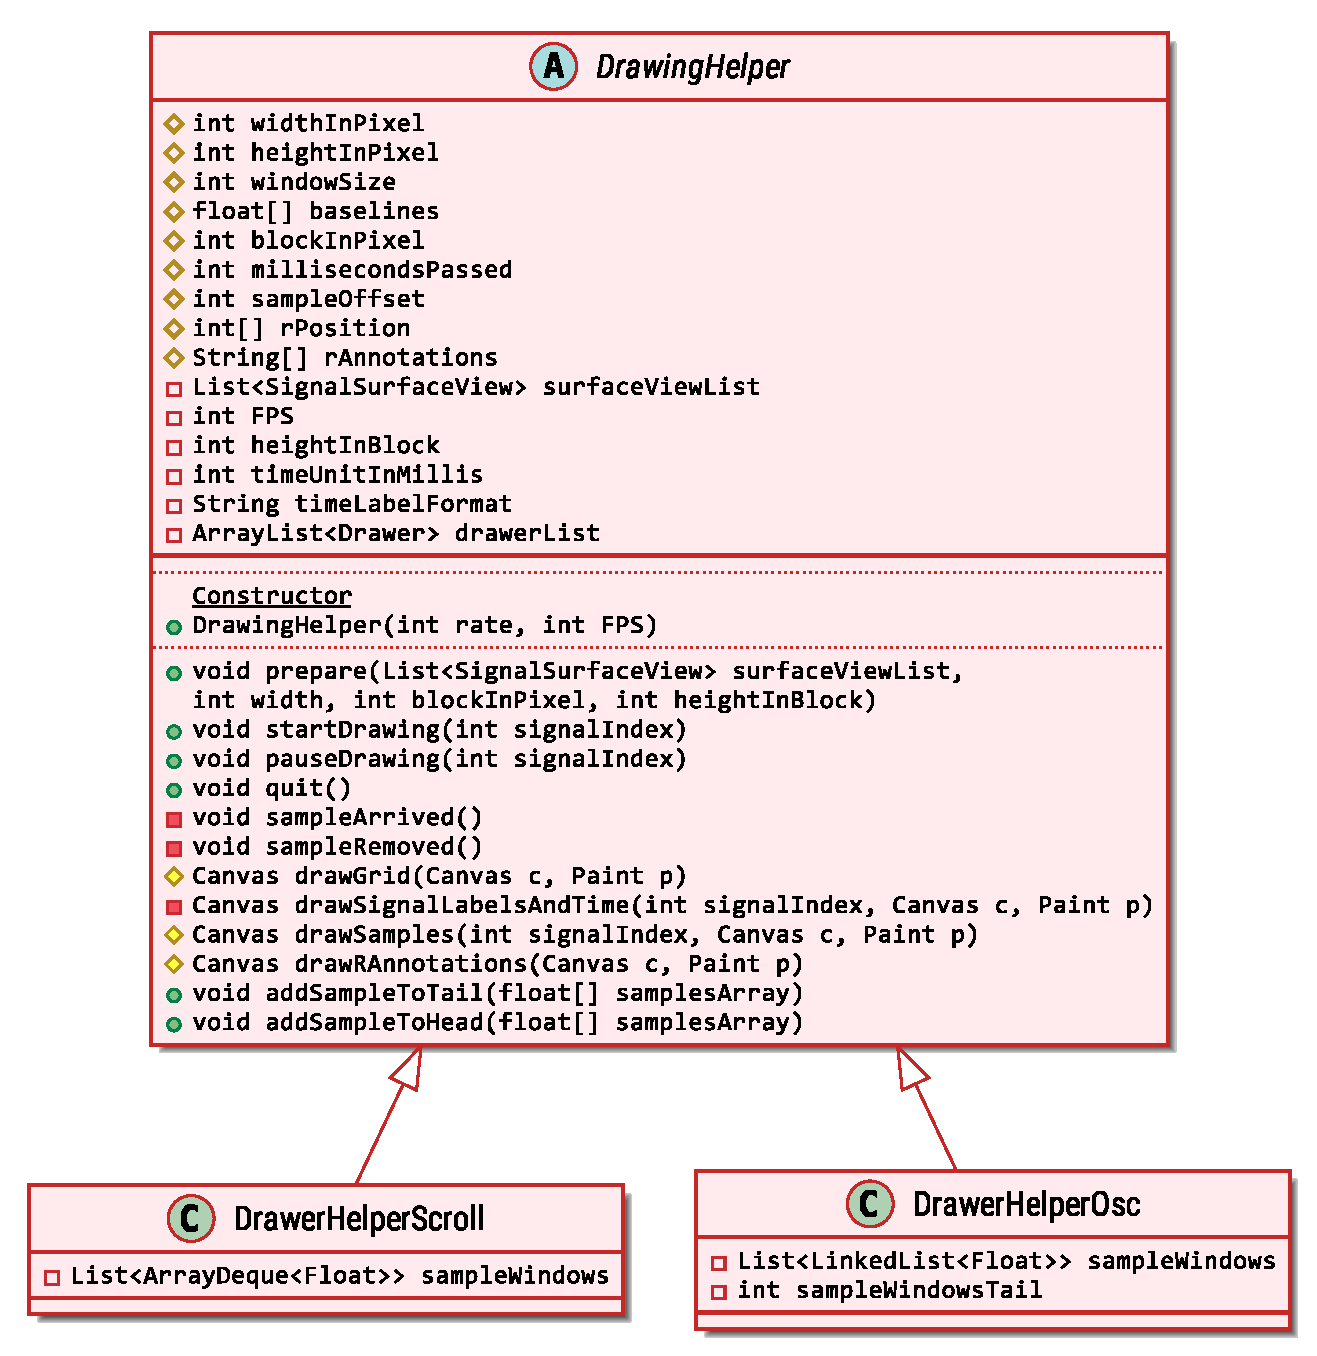
\includegraphics[width=140mm]{figures/ch9/10.eps}
	\caption{Class diagram of the DrawingHelper class.}
	\label{fig9.10}
\end{figure}

\subsubsection{Drawer}
As already mentioned earlier, the Drawer class will be a thread, responsable of drawing on one or more SignalSurfaceViews. It is a private static inner class of the DrawingHelper, and it hold a WeakReference to the DrawingHelper in order to avoid as much as possible memory leaks.\cite{ref26} It extends the HandlerThread class and its basic functioning is reading and responding to all messages sent to its MessageQueue. The messages will contain the index of the ECG lead that need to be drawn. Actually, there will be always only one message per ECG lead on its MessageQueue: this is because, beside of the lead index, all messages are equals, and incorporate the same drawing routine including all drawing method seen in the previous section. But each message at the end will also include a recursive sending of the next message to the MessageQueue, delayed by the time unit dictated from the specified FPS of the application. So each message will cause a sending of the next message. In this way, the Drawer we can continuously draw and update the SignalSurfaceView, at a rate of FPS. The starting of drawing will be managed by the DrawingHelper, which will send the first recursive message. The pausing, manage by the same, will be easily achieved by the removal of all the messages present in the MessageQueue at that moment.\\
In the figure \ref{fig9.11} is showed the class diagram of the Drawer.
\begin{figure}[ht!]
	\centering
	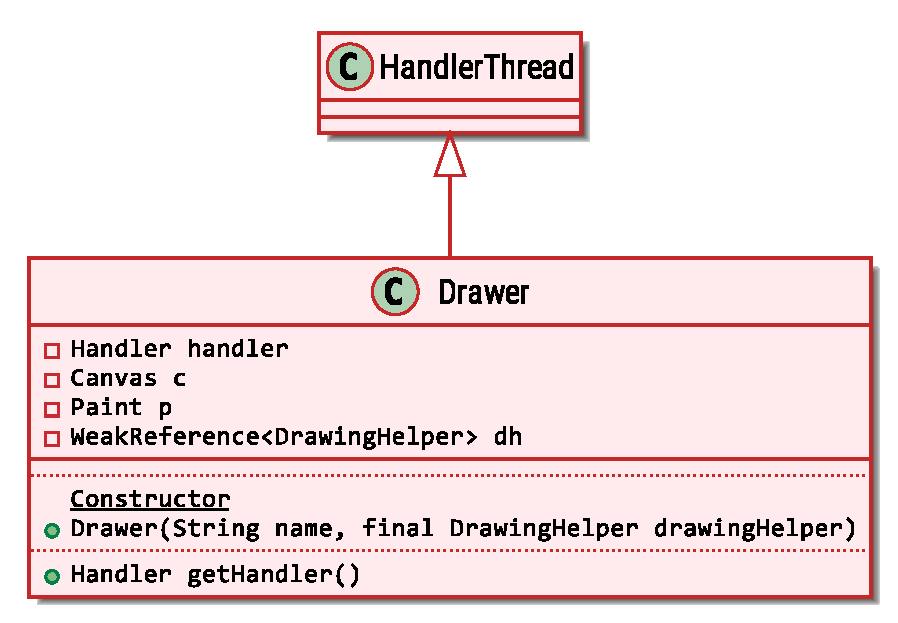
\includegraphics[width=100mm]{figures/ch9/11.eps}
	\caption{Class diagram of the Drawer class.}
	\label{fig9.11}
\end{figure}

\subsection{Connection}
As we have often mentioned, the communication between the acquisition device and the app will rely on a bluetooth connection. There are mainly two different situation where we are using this type of connection:
\begin{itemize}
	\item During the device connection menu, where we use bluetooth to scan all nearby devices in order to find ZEcg;
	\item During real-time acquisition, when we are connect to the device and start receiving the patient ECG samples.
\end{itemize}
In the first case, we made use of a BroadcastReceiver, which will be notified during bluetooth scanning, when a new device will be found. As we don’t want to include external devices in the device scan list, we filtered all devices by name, and included only devices with a name containing the word \textit{“ecg”}.\\
In the second case we made use of the class BluetoothSerial, which is an external library that we have modified and included in our application. The type of connection between two devices differs according to the specific bluetooth modules mount on the different devices we tested our application with. For most of the devices we could establish an unsecure connection with Zecg, without any  security protocols nor explicit  pairing request. On other devices the connection was established only after an explicit pairing request. Either way the Zecg was always the server side and the smartphone the client side of the Bluetooth connection. Whenever a client closes the connection with the server, the connection is automatically lost and any other device can ask data from the server.

\subsubsection{BluetoothSerial}
As we have said when we were talking about the ZEcgReceiver, the BluetoothSerial class will pass data received from the acquisition device to the last by sending messages to it. This is done by using an Handler instance that is passed in the BluetoothSerial constructor, that is pointing to the MessageQueue of the ZEcgReceiver. The messages will include the partial data received from the bluetooth connection, that will be parsed as we described in the ZEcgReceiver section. BluetoothSerial will create different thread, where each one will handle a different connection step:
\begin{itemize}
	\item AcceptThread: this thread runs while listening for incoming connections. It behaves like a server-side client. It runs until a connection is accepted (not used in our case, as the smartphone always act like a client in the connection);
	\item ConnectThread: this thread runs while attempting to make an outgoing connection with a device. It runs straight through. The connection either succeeds or fails;
	\item ConnectedThread: this thread runs during a connection with a remote device. It handles all incoming and outgoing transmissions (only incoming in our case).
\end{itemize}
In the ConnectedThread the message sending will take place.

\subsection{Operations Flow}
In the previous sections we went deep to some component implementations in order to clarify some of the main functioning and iterations. Therefore, we move from a low level description, to an higher level, in order to explain the flow of the app operations. We will focus on our main two operation flow:
\begin{itemize}
	\item Record acquisition: the user acquires a new ECG record by connecting to the acquisition device;
	\item Saved record opening: the user open a stored ECG record, choosing one of them from a list, and visualizes it.
\end{itemize}
For the sake of clarity, we put aside technical terminology for activity describing, as some methods call may be not so explanatory for the understanding. Instead, we used a general description of each activity, being all the details in the previous sections.

\subsubsection{Record acquisition}
\begin{figure}[ht!]
	\centering
	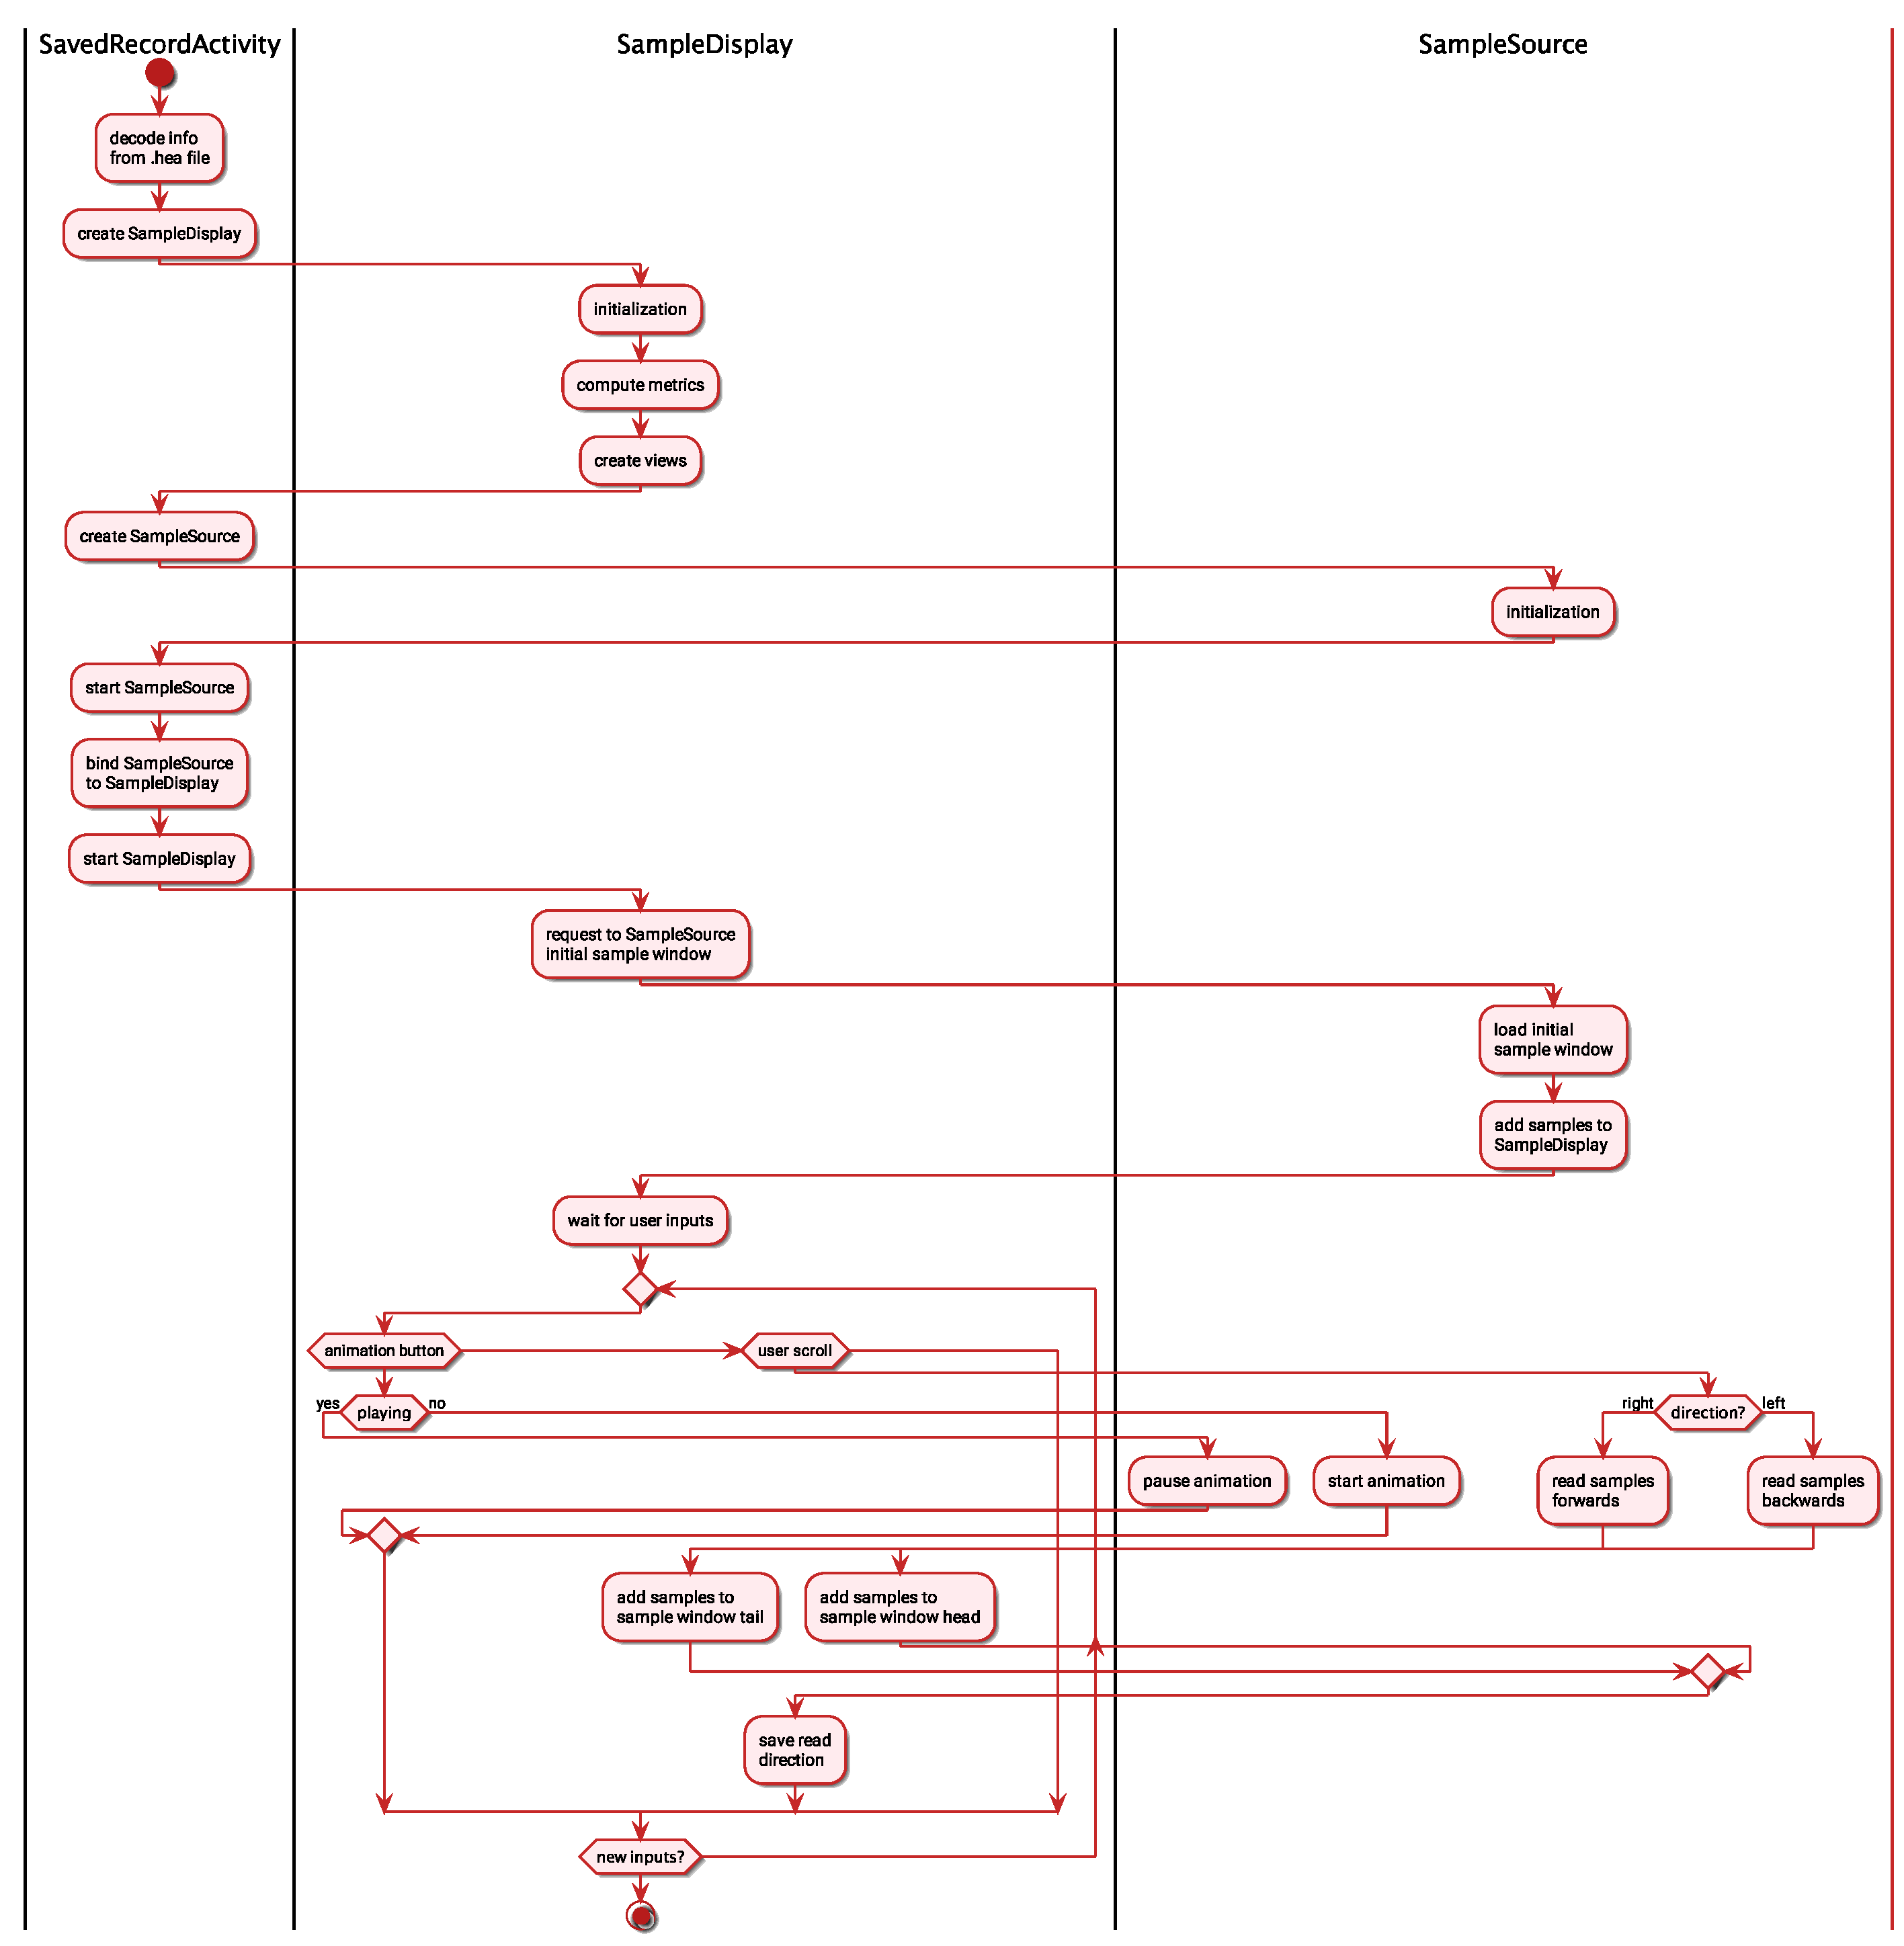
\includegraphics[width=\linewidth]{figures/ch9/12.eps}
	\caption{Activity diagram of a new ECG record acquisition operation.}
	\label{fig9.12}
\end{figure}
The process starts with the selection of \textit{“New Record”} in the app home. After that the user will move to the CreateNewRecordActivity, where will be displayed a form where the user will be required to specify his:
\begin{itemize}
	\item Name,
	\item Surname,
	\item Sex,
	\item Age,
	\item Weight.
\end{itemize}
If the user will omit some information, and clicks on the submit button, an error will be displayed, asking the user to complete the form. After a positive check of the form, there will be the creation of the .hea, including all the previous user data, and the .dat file, the container of all ECG record samples.\\
Then, the bluetooth connection of the device will be checked: if deactivated, the user will be jumped to the DeviceConnectionActivity, where will be able to activate it and search for the acquisition device; if activated, the BluetoothSerial will start the connection with the device, and wait for the first data. At each new data arrival, it will send a message with the new data to the ZEcgReceiver class. This last after having received the message, will extract the new data and insert it into a acquisition buffer. Then it will try to empty the buffer, removing all complete samples. All removed sample will be decoded and added to the sample window tail of the SampleDisplay.
The process of acquiring new data and pass it to the ZEcgReceiver continues until the user will click on the stop button. Afterwords, the connection will be close and additional data will be written to the .hea record file. The operations flow are depicted as an activity diagram in the figure \ref{fig9.12}.

\subsubsection{Saved record opening}
\begin{figure}[ht!]
	\centering
	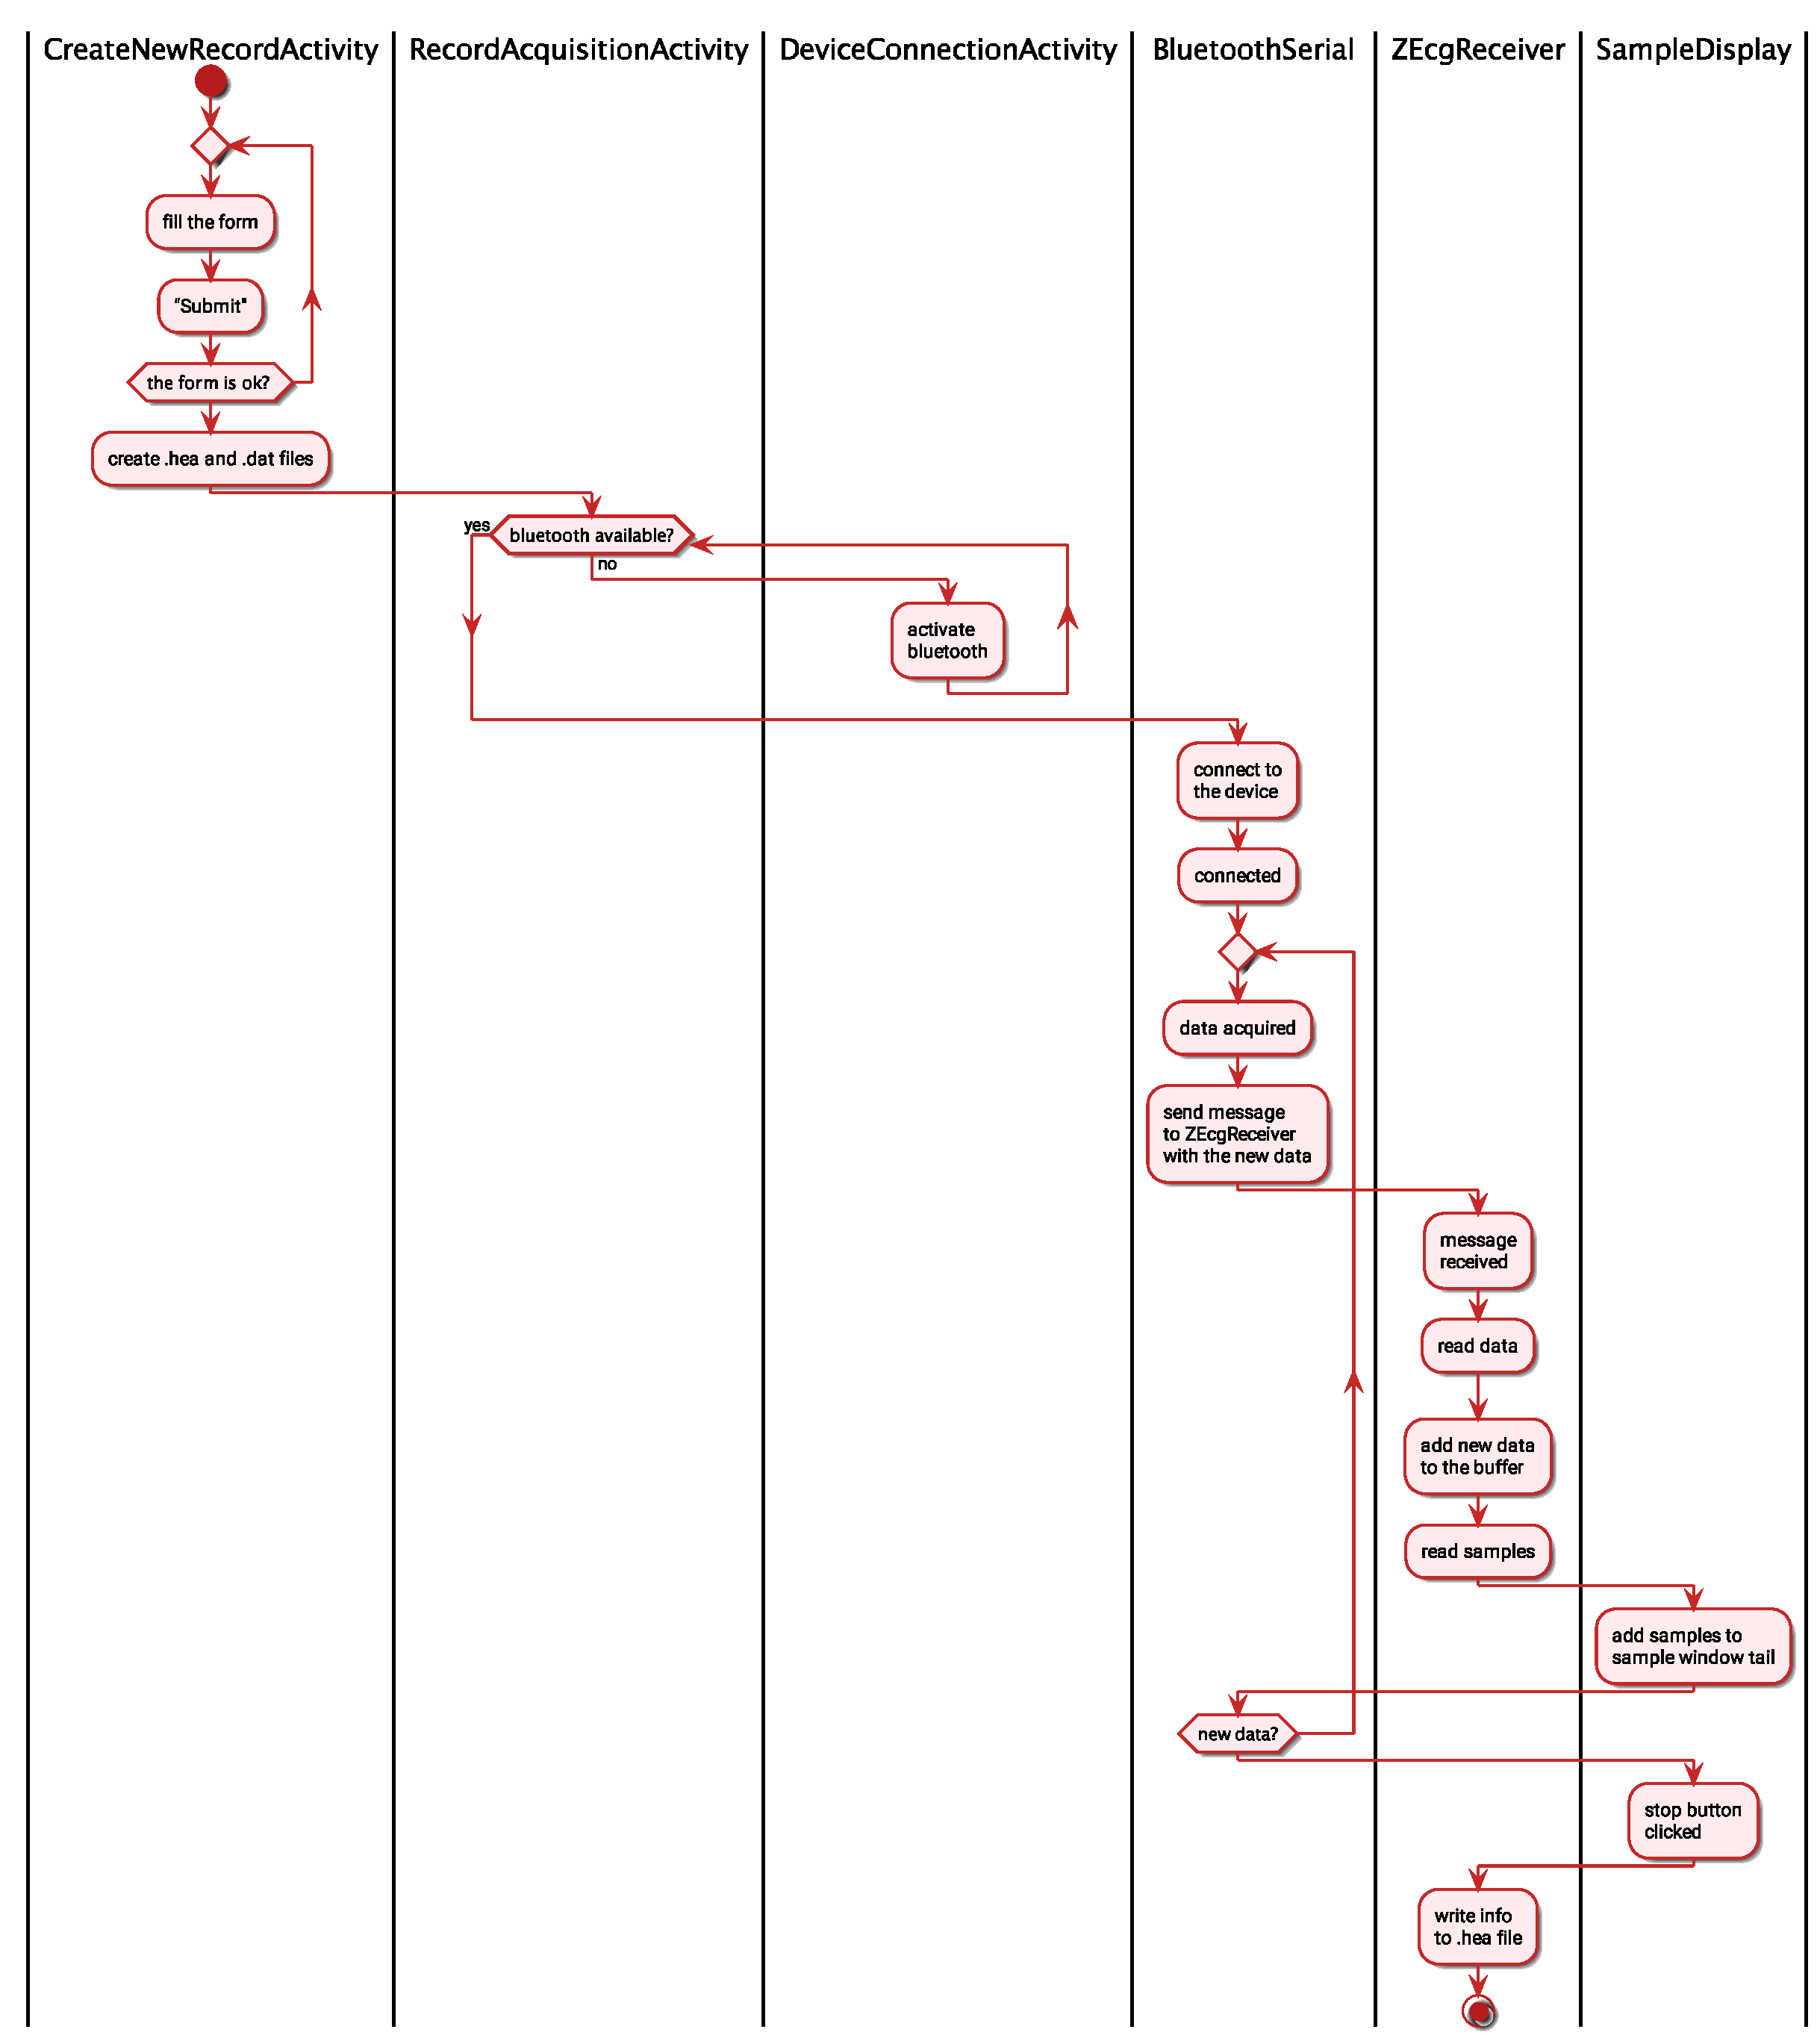
\includegraphics[width=\linewidth]{figures/ch9/13.eps}
	\caption{Activity diagram of a new ECG record acquisition operation.}
	\label{fig9.13}
\end{figure}
The process starts with the selection of \textit{“Open Record”} in the app home. A list of all stored ECG record will be presented to the user. The user will be able to scroll the list and select a ECG record to open it. After that it will be moved to the SavedRecordActivity, where the record .hea file will be decoded to extract all useful information, as sample rate, number of lead, lead labels, signal gain and others. Then, the SampleDisplay component will be created: this will compute all the metrics for which regarding the dynamic ECG paper sizing, and will create all ECG paper strip views. Subsequently, the SampleSource will be created and initialized and binded to the SampleDisplay, which will be started. At start, the SampleDisplay will request from the SampleSource the initial sample window, in order to fill the ECG lead strips created previously. Later, the SampleDisplay will start waiting for any user input. The user input will be of two types:
\begin{itemize}
	\item Animation button click;
	\item Scrolling.
\end{itemize}
In the first case, the state of the animation will be queried:
\begin{itemize}
	\item If playing, the animation will be stopped;
	\item Otherwise, the animation will be started.
\end{itemize}
In the second case, according to the scrolling direction, the respective samples will be read and added to sample window tail or head, respectively if right or left.\\
The process of processing new user inputs continues until the user will close the record visualization. The operations flow are depicted as an activity diagram in the figure \ref{fig9.13}.